SpiderMonkey is the JavaScript Engine for Mozilla, an extremely widely
used, security-critical interpreter/JIT compiler.  SpiderMonkey has
been the target of aggressive random testing for many years now.  A
single fuzzing tool, \texttt{jsfunfuzz} \cite{jsfunfuzz}, is
responsible for identifying more than 1,700 previously unknown bugs in
SpiderMonkey \cite{jsfunfuzzbugs}.  SpiderMonkey is (and was) very
actively developed, with over 6,000 code commits in the period from
1/06 to 9/11 (nearly 4 commits/day).  SpiderMonkey is thus ideal for
evaluating how reduction aids localization when using a sophisticated
random testing system, using the last public release of the
\texttt{jsfunfuzz} tool \cite{jsfunfuzz}, modified for swarm testing \cite{ISSTA12}.
Using a set of faults in SpiderMonkey version 1.6 found with random
testing in previous research \cite{PLDI13}, we show that reduction is
essential for localization of bugs found using random testing, and
that the use of reduction is even somewhat more important than the
choice of localization formula.  


\begin{table}
\begin{center}
\begin{tabular}{|c||c|c|c|c|c||c|c|c|c|c|}
%\hline
\hline
Bug\# & Revision Fixed &  \#Failures & {\tt diff} size \\
\hline
\hline
{\tt R60} & 1.16.2.1 & 1 & 115  \\
\hline
{\tt R95} & 1.3.2.3.8 & 7 & 111   \\
\hline
{\tt R115} & 1.4.8.1 & 4 & 592   \\
\hline
{\tt R360} & 3.117.2.6 & 3 & 223  \\
\hline
{\tt R880} & 3.17.2.14 & 28 & 272   \\ 
\hline
{\tt R1172} & 3.208.2.63 & 150 & 214  \\
\hline
{\tt R1294} & 3.241.2.1 & 405 & 80  \\
\hline
{\tt R1543} & 3.36.16.1 & 146 & 169  \\
\hline
{\tt R1561} & 3.37.2.1.4.1.2.2 & 2 & 31  \\
\hline
{\tt R1873} & 3.50.2.29 & 1,041 & 56  \\
\hline
%\hline
\end{tabular}
\end{center}
\caption{Spidermonkey Bugs}
\label{tab:spiderbugs}
\end{table}


\begin{figure*}[t]
  \centering
  %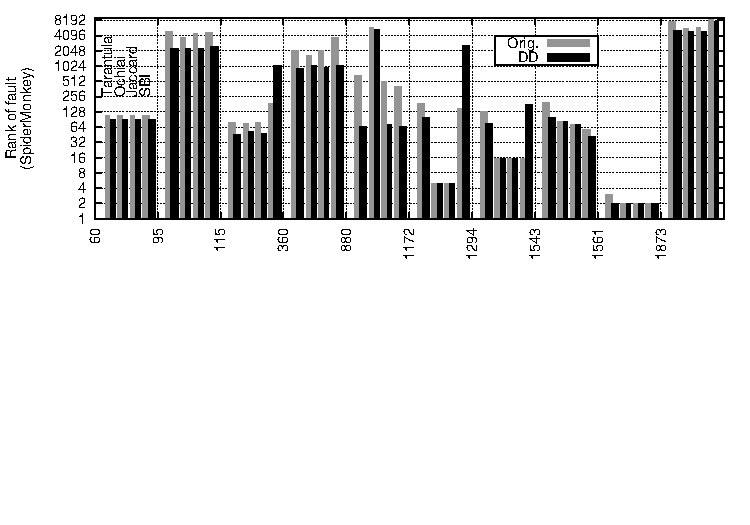
\includegraphics[width=2\columnwidth]{naspidermonkey}
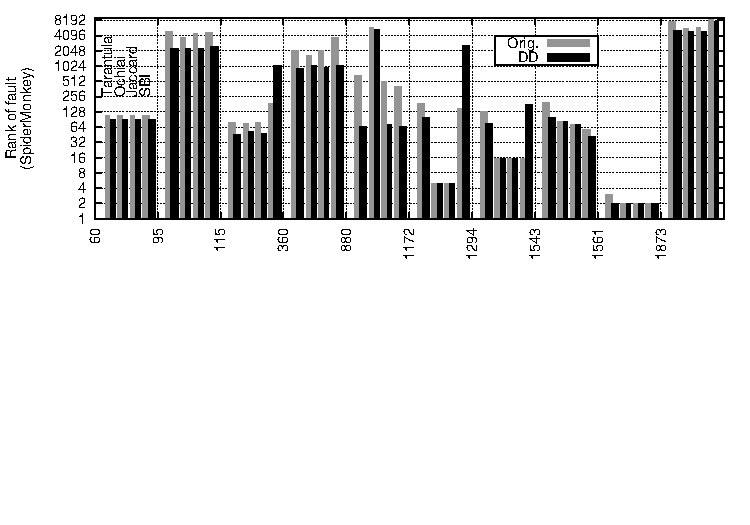
\includegraphics[scale=1.1]{naspidermonkey} 
 \vspace{-2in}
  \caption{SpiderMonkey Results}
  \label{fig:spidermonkey}
\end{figure*}

Figure \ref{fig:spidermonkey} shows the change in rankings of the
faulty code for 10 SpiderMonkey bugs (Table \ref{tab:spiderbugs}).
These bugs were taken from our PLDI 2013 data set \cite{PLDI13}.  Out
of the 28 bugs studied in that paper we chose 10 random bugs for which, by
hand, we could confirm the true set of faulty lines in the code
commit.  Each bug is identified by the revision number of the commit
in which it was fixed: e.g., R0 maps to revision 1.10.4.1, the first
commit of Spidermonkey changes under consideration. Table
\ref{tab:spiderbugs} shows all bugs studied, the commit version fixing
the bug, the number of failing test cases for that bug (\# Failures),
and the size (in lines) of the fixing commit's {\tt diff}.  The faults
under consideration here are clearly non-trivial (in fact, most fixes
involved changes to multiple source files).  For our localization we
used the original and reduced test cases from PLDI 13 \cite{PLDI13}
plus 720 additional randomly generated \emph{passing} tests generated
using the same tool.

Across these 10 bugs, the average ranking for the first faulty line
encountered was 1,550.7 without reduction, improving to 994.5 with
reduction.  Reduction improved the localization in 33 cases, with a
minimum improvement of 1 ranking and a maximum improvement of 2,137
positions.  The average improvement was 674 positions.  The results
were unchanged in 7 cases. It is important to note that even with such
a challenging setting and real bugs, fault localization with reduction
performs better then fault localization without reduction irrespective
of formula being used: in the \emph{worst} case it performed equally well. It was better to use reduction than to optimally (from worst to
best) switch formula for 5 of the 10 bugs; it was better to switch
formula in 4 cases, and in one case both methods gave the same result.
While the results show that reduction was extremely effective in
improving localization, it is also true that the localization was
\emph{still not very helpful} in many of these cases, considering absolute pessimistic rank as success criteria.  Of course,
SpiderMonkey 1.6 has over 80KLOC, and even reduced failing tests
typically executed over 8,000 lines of code, so a ``poor''
localization may be useful in such a large fault search space.  For 6
of the 10 bugs, all scores after reduction gave a fault ranking $< 128$.

